
\section{Cup Holder}
One of the challenges a wheelchair user faces is carrying objects while having
to propel the chair. In order to solve this problem, we have installed a
carrying mechanism: a cup holder. This subsystem consist of a foam cup holder
attached to the top of the arm of the wheelchair with duct tape. It allows the
user to carry small objects without the need to use their hands, freeing them
to spin the drive wheels.

\subsection{Technical Specifications}
This subsystem must be attached firmly so it doesn't slide sideways and end up
under the chair arm. It is created using a foam cup holder, scissors, and a
roll of tape (duct tape is used here). The scissors are used to cut a slit in
two opposite sides of the cup holder, slits long enough to fit the tape
through. A portion of the tape should be folded over on itself so it doesn't
stick to the cup holder while it is attached. The tape is then pushed through
the cup holder so the folded over portion sticks out the opposite end and the
sticky side is still on the original side. The cup holder is then taped tightly
to the arm of the chair. Either arm is acceptable.

\begin{table}[H]
    \centering
    \label{tbl:cupholder-cost}
    \caption{Cup Holder Cost Analysis}
    \begin{longtable}{l c l}
        Description & Quantity & Estimated Cost \\
        \hline
        Foam Cup Holder & 1 & 0.27 -- 0.52 USD\cite{cost-cupholder} \\
        Scissors & 1 per worker & Negligible \\
        Duct Tape of $\leq 50$ $mm$ width & $\sim 250$ $mm$ & 0.01
        USD\footnotemark[1] \\
        Labor Cost & $\sim 1$ $min$ & 0.00 USD\footnotemark[2] \\
        \hline
        \multicolumn{2}{r}{Estimated cost per chair} & 0.28 -- 0.53 USD
    \end{longtable}
\end{table}
\footnotetext[1]{The labor cost per chair is negligible as this will be done by volunteers.}
\footnotetext[2]{The cost of tape per chair was determined by finding the
            cost of a roll of 18288~$mm$ of duct tape ($\sim$3.50~USD) and applying
            this to an estimated length per chair. This length was intentionally overestimated.}
\subsection{Client Requirements}
This subsystem addresses the concern of users ability to carry objects. It
gives them a convenient place to carry small objects.

During the user empathy activities and the client's presentation, this
topic appeared often. People in Africa are expected to provide for
themselves as much as possible, and being able to carry necessary objects
or fluids reliably is a step in that direction. Often, wheelchair users
place objects in their laps to carry them. They cannot usually grip these
objects, however, as they usually have little power over their legs. This
is especially common with very large or very small objects. This cup holder
addresses the problem of carrying small objects.

\subsection{Relation to Other Subsystems}
The cup holder works with the seat belt to allow for carrying objects. While
the cup holder allows the user to carry small objects, the seat belt allows the
user to carry larger objects. Together, these subsystems solve the problem as
completely as possible.

\begin{figure}[H]
    \label{fig:cupholderasm}
    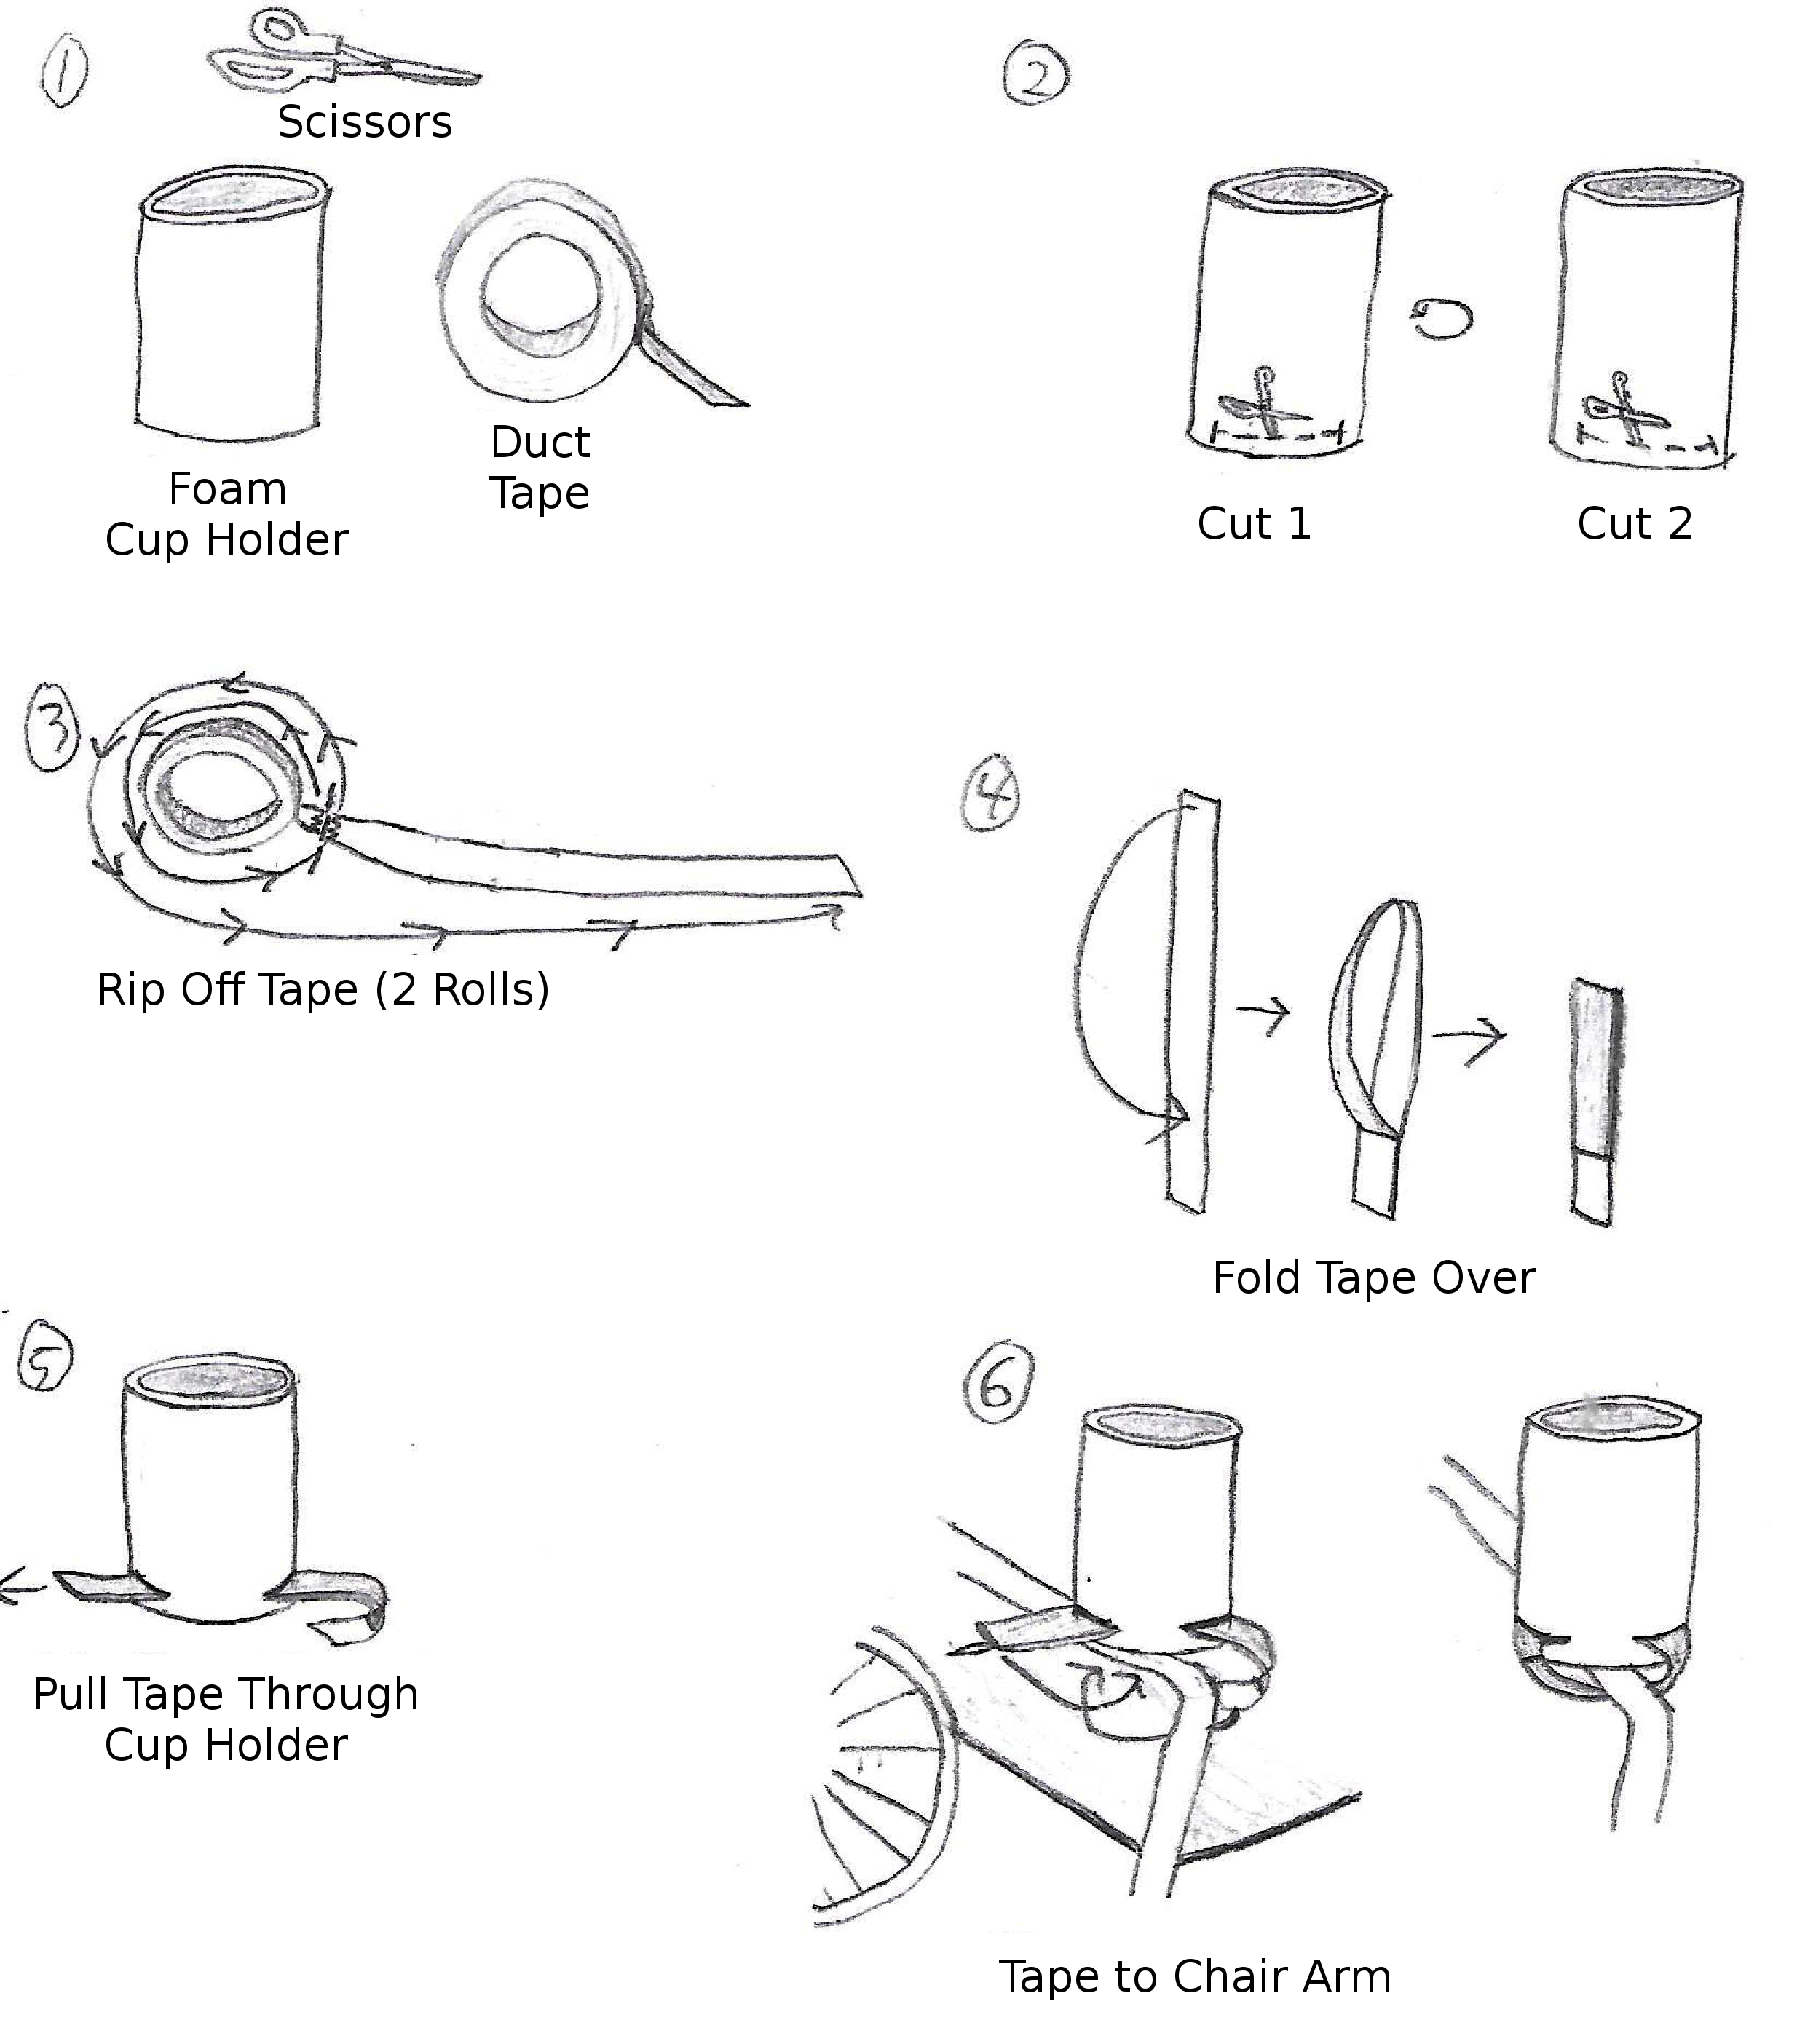
\includegraphics[width=\textwidth]{cupholderasm}
    \caption{Illustrated Assembly for the Cup Holder}
\end{figure}
